\subsection{Interazioni}
\begin{itemize}
    \item L'interazione classica a distanza è descritta da un potenziale o da un campo. In meccanica quantistica invece c'è uno scambio di quanto, e ad ogni interazione è associato un bosone.
    \item Ad esempio consideriamo due cariche. Classicamente la forza che la prima carica esercita sulla seconda dipende dal campo elettrico; quantisticamente invece l'interazione tra le due cariche è mediata da un fotone, figlio della violazione di conservazione di energia in accordo con il principio di indeterminazione di Heisenberg $\Delta E\Delta t\sim\hbar$.
    \item Esistono quattro tipi di interazione: 
    \begin{enumerate}
        \item Forte. Lega i quark in adroni e protoni/neutroni in nuclei. È mediata dai gluoni.
        \item Elettromagnetica. Lega gli elettroni al nucleo formando l'atomo ed è anche responsabile delle forze molecolari in liquidi e solidi. È mediata dai fotoni.
        \item Debole. È responsabile dei decadimenti radioattivi, specie i $\beta$-decay. È mediata dai bosoni W e Z.
        \item Gravitazionale. È la più debole e riguarda ogni corpo con massa. È mediata dai gravitoni... o forse no.
    \end{enumerate}
    \item Come sappiamo la massa del mediatore è inversamente proporzinale al range della interazione. Se il mediatore ha massa nulla, il range è infinito (fotone ed interazione elettromagnetica). Se il mediatore ha massa finita, il range è finito. Più è massivo, più è corto il range. Infatti la interazione debole ha range molto piccolo (inferiore al fermi) e il mediatore lo metto in evidenza solo ad energie elevate.
    \item Per indicare l'intensità di ciascuna forza (non ho letto sbene slide diceva di protoni che si toccano) si pone pari a uno l'interazione forte. Allora avremo \\
    \begin{tabular}{>{\centering\arraybackslash}m{3cm} >{\centering\arraybackslash}m{3cm} >{\centering\arraybackslash}m{3cm} >{\centering\arraybackslash}m{3cm}}
        Forte & Elettromagnetica & Debole & Gravitazionale \\
        1 & $10^{-2}$    & $10^{-7}$    & $10^{-39}$    \\
    \end{tabular}\\
    Secondo Einstein forse è possibile unificare le quattro forze in un'unica teoria, ma non è ancora stato fatto. Finora solo la forza elettromagnetica e debole sono state unificate in una sola teoria. Si pensa che ad alte energie si riescono a unificare tutte le forze, solo che sono troppo elevate per raggiungerle. A $10^{16}$ GeV si uniscono forza elettromagnetica, debole e forte; A $10^{19}$ GeV si unisce anche la gravitazionale. Oggi siamo a 12 ordini di grandezza di distanza da $10^{16}$ GeV. 
    \item L'intensità di una forza è associata ad una costante di accoppiamento.
    \begin{enumerate}
        \item Quella elettromagnetica sappiamo che è la costante di struttura fine
        \begin{equation*}
            \alpha=\frac{\text{Energia elettrostatica tra due elettroni a distanza }\hbar/mc}{\text{massa a riposo dell'elettrone}}=\frac{\frac1{4\pi}\frac{e^2}{\hbar/mc}}{m_ec^2}=\frac{e^2}{4\pi\hbar c}=\frac1{137}
        \end{equation*}
        \item Quella debole interviene nei $\beta$-decay e in assorbimenti di neutrini (che sarebbe la stessa cosa). Ma interviene anche in altri processi più \textit{strani}. Vediamo i due decadimenti:
        \begin{equation*}
            \underset{dds}{\Sigma^-}\to \underset{ddu}{n}+\pi^-\qquad \tau_w\sim10^{-10}s\qquad \text{Forza debole}
        \end{equation*}
        \begin{equation*}
            \underset{uds}{\Sigma^0}\to \underset{uds}{\Lambda}+\gamma\qquad \tau\_{EM}\sim10^{-19}s\qquad \text{Forza elettromagnetica}
        \end{equation*}
    La prima è effettivamente associata all'interazione debole in quanto viene violata la conservazione di flavour (un quark strange diventa up) ed ha un tempo di $10^{-10}$s, mentre la seonda è elettromagnetica perché, oltre alla presenza di un fotone, viola soltanto la conservazione dell'isospin e il tempo è di $10^{-19}$s. Come già sappiamo, il principio di indeterminazione lega vita media e larghezza del decadimento in modo inversamente proporzionale. Ma anche la larghezza di decadimento $\Gamma$ dipende dalla costante di accoppiamento $\alpha$ che caratterizza l'interazione tra lo stato iniziale e i prodotti finali del decadimento. In generale, il tasso di decadimento (sezione d'urto) è proporzionale al quadrato della costante di accoppiamento, quindi possiamo scrivere che $\Gamma\propto\alpha^2$. Questa dipendenza dal quadrato della costante di accoppiamento è una conseguenza della teoria quantistica dei campi, dove l'ampiezza della transizione dipende linearmente da $\alpha$, mentre la probabilità di transizione (e quindi il tasso di decadimento o sezione d'urto) dipende dal modulo al quadrato di tale ampiezza. Da ciò segue che il tempo di vita medio $\tau$ è inversamente proporzionale al quadrato della costante di accoppiamento $\alpha$: $\tau\propto\alpha^{-2}$ di conseguenza, più è forte l'interazione (cioè, maggiore è la costante di accoppiamento), più breve sarà il tempo di vita della particella, mentre un'interazione più debole (con $\alpha$ più piccolo) darà luogo a un tempo di vita più lungo.
    \begin{equation*}
    \frac{\alpha_w}{\alpha}=\sqrt{\frac{\tau\_{EM}}{\tau_w}}\approx 10^{-4}-10^{-5}
    \end{equation*}
    Cioè, come già visto nella tabella precedente, la forza debole è 4-5 ordini meno intensa di quella elettromagnetica.
    \item L'interazione forte invece conserva tutto. Quindi quella elettromagnetica viola al massimo la conservazione di isospin; quella debole viola molte cose tra cui parità, coniugazione di carica, flavour ed isospin; quella forte non viola niente. Vediamo le due reazioni:
    \begin{equation*}
        \Sigma^{0*}(1385)\to\Lambda+\pi^0\qquad\tau\sim10^{-23}s\qquad{\text{Forza forte }}\Gamma=36\MeV
    \end{equation*}
    \begin{equation*}
        \Sigma^0(1192)\to\Lambda+\gamma\qquad\tau\sim10^{-19}s\qquad{\text{Forza elettromagnetica}}
    \end{equation*}
    In questo caso abbiamo 
    \begin{equation*}
    \frac{\alpha_s}\alpha=\sqrt{\frac{\tau\_{EM}}{\tau_s}}=\sqrt{\frac{10^{-19}}{10^{-23}}}\approx10^2
    \end{equation*}
    I quanti in questo caso sono i gluoni e ci sono sei cariche. La forza tra i quark è simmetrica per colore ossia non dipende da essa. Vale la cromodinamica quantistica per l'interazione forte, e si hanno i due comportamenti: 
    \\
    \begin{center}
    \begin{tabular}{>{\centering\arraybackslash}m{3cm} >{\centering\arraybackslash}m{3cm} >{\centering\arraybackslash}m{3cm}}
        Libertà asintotica & $V_s\to\alpha_s/r$ & $q^2\to\infty$\\
        Confinamento & $V_s\to kr$ & $q^2\to0$\\
    \end{tabular}\\
    \end{center}
    Cioè ad alte energie (piccole distanze) il potenziale è coulombiano, mentre a piccole energie (grandi distanze) il potenziale è elastico. La soglia di energia alta/bassa è sui GeV.
\end{enumerate}
\end{itemize}
\subsection{Diagrammi di Feynman}
Introduzione inutile sui diagrammi. Lei però considera tempo da sinistra verso destra. Dice anche la storia dell'interferenza di quando consideri più diagrammi per uno stesso processo (fai il quadrato della somma, non la somma dei quadrati quella storia lì perché i diagrammi sono ampiezze).
\subsubsection{Variabili di Mandelstam}
Consideriamo il processo $a+b\to c+d$ (e.g. $p\bar p\to n\bar n$). Le variabili di Mandelstam sono (per processi $2\to2$):
\begin{enumerate}
    \item $s=(p_a+p_b)^2=(p_c+p_d)^2$ è il quadrato dell'energia nel centro di massa.
    \item $t=(p_a-p_c)^2=(p_b-p_d)^2$ è il quadrato del momento trasferito.
    \item $u=(p_a-p_d)^2=(p_b-p_c)^2$ è il quadrato del momento scambiato.
\end{enumerate}
Inoltre vale $s+t+u=(m_a^2+m_b^2+m_c^2+m_d^2)$ è la somma delle masse a riposo.
\begin{itemize}
    \item Facciamo un esempio con lo scattering elettrone-positrone, quindi supponendo $E_i\sim p_i$. Nel riferimento del centro di massa avremo:
    \begin{equation*}
    \begin{cases}
        p_a=(E,p,0,0)\\
        p_b=(E,-p,0,0)\\
        p_c=(E,p\cos\vartheta,p\sin\vartheta,0)\\
        p_d=(E,-p\cos\vartheta,-p\sin\vartheta,0)
    \end{cases}
    \end{equation*}
    con $\vartheta$ l'angolo tra la direzione iniziale di collisione e la direzione di scattering (finale). Allora abbiamo:
    \begin{equation*}
        \begin{cases}
            s=4E^2\text{ come nei collider}\\
            t=-\frac12s(1-\cos\vartheta)=-s\sin^2\frac\vartheta2 \\
            u=-\frac12s(1+\cos\vartheta)=-s\cos^2\frac\vartheta2
        \end{cases}
    \end{equation*}
        e si ha effettivamente $s+t+u=0$, che vuol dire che solo due variabili sono indipendenti e scegliamo noi quale usare per descrivere il sistema (e.g. $(E,\vartheta)$,$(s,t)$, $(\sqrt s,\vartheta)$). Invece l'angolo azimutale $\varphi$ non compare e c'è simmetria (della sezione d'urto) in esso se la dinamica non lo esplicita, ad esempio con lo spin. Se non posso trascurare la massa $s=m_a^2+m_b^2+2p_ap_b\implies s+t+u=\sum_i m_i^2$.
        \item Consideriamo adesso masse uguali. Diamo una rappresentazione grafica o qualcosa del genere non è che si capisce a che cosa serva.
        \begin{equation*}
            \begin{cases}
                s=4E^2\geq 4m^2\\
                t=-4p^2\sin^2\frac\vartheta2 \\
                u=-4p^2\cos^2\frac\vartheta2
            \end{cases}
        \end{equation*}
        L'equazione $s+t+u=4m^2=M$ oltre a dirci che solo due variabili sono indipendenti, rappresenza l'equazione di un piano nello spazio 3D $stu$. La regione del piano in cui $s,t,u>0$ forma un triangolo equilatero, come in \autoref{fig:mandelstam}.
        \begin{figure}[h]
            \centering
            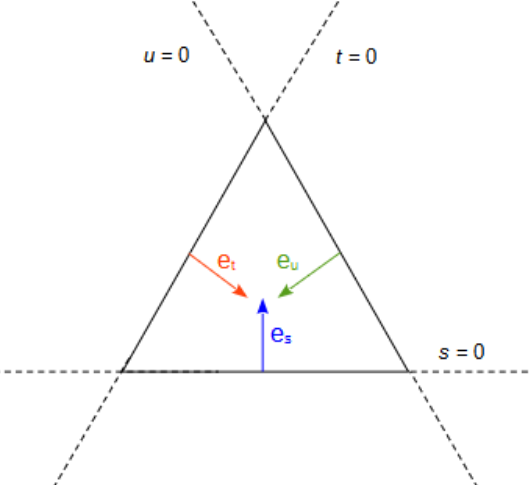
\includegraphics[width=0.45\textwidth]{immagini/fig_mandelstam.png}
            \caption{Piano di Mandelstam}%Ragazzi non ne ho idea è più comprensibile il corso di Greco.}
            \label{fig:mandelstam}
          \end{figure}
          I confini di questo triangolo sono dati dalle linee \( s = 0 \), \( t = 0 \) e \( u = 0 \), come mostrato. Il vertice superiore del triangolo corrisponde a \( t = u = 0 \), quindi, dalla equazione precedente, vediamo che l'altezza del triangolo è \( M \). Sebbene siano necessari solo due vettori unitari per specificare una posizione in questo piano, è consuetudine definire tre vettori unitari \( \vec{e}_s \), \( \vec{e}_t \) e \( \vec{e}_u \), ciascuno dei quali è perpendicolare alla rispettiva linea zero, come mostrato in \autoref{fig:mandelstam}. Visto che l'angolo tra due di questi versori è sempre $\frac23\pi$, abbiamo 
          \begin{equation*}
          \vec{e}_i\cdot\vec{e}_j=\cos\frac23\pi=-\frac12 \qquad i\neq j
          \end{equation*}
          Per qualche motivo oscuro vogliamo esprimere ${\vec e_i}$ in funzione di $\hat x$ e $\hat y$. Notiamo subito che $\vec e_s=\hat y$. Invece $\vec e_u$ ha un angolo pari a $\frac23\pi+\frac\pi2=\frac76\pi$ rispetto all'asse $\hat x$, dunque $\vec e_u=(-\frac{\sqrt3} 2,-\frac12)$. Infine $\vec e_t$ sta a $-\frac\pi6$ rispetto all'asse $\hat x$, quindi $\vec e_t=(\frac{\sqrt3}2,-\frac12)$. Queste relazioni possiamo invertirle e ricavare $\hat x$ e $\hat y$ in funzione di $\vec e_i$. Riprendi appunti e parla di regioni permesse.
\end{itemize}